\chapter{Training Strategy using Evolutionary Algorithm}
\label{chap:Five}
\section{Introduction}
\label{sub:five-intro}
This chapter covers an overview on the contribution of Dr M Jones
of the Axelrod-Python library. Following the presentation of Axelrod-Python
library at PyConUk 2015~\url{http://2016.pyconuk.org/}, he became a member of
the Axelrod-Python team and contributed to the library a new strategy, the
EvolvedLookerUp, which is currently ranked second in the Axlerod-Python tournament.
EvolvedLookerUp is a LookerUp strategy that uses a lookup table trained using an
evolutionary algorithm. The structure of the strategy and the evolutionary algorithm
will be covered in the following sections.

Furthermore, the method developed by M Jones to train the EvolvedLookerUp
will be redeveloped and used. Making it possible to train a new strategy
by competing against random opponents in various spatial tournaments.


\section{The Lookup Evolve Algorithm}
\label{sub:lookup-evolve-algorithm}
As stated in ~\autoref{sub:five-intro}, the LookerUp strategies uses a lookup to
determine the strategy's next move. In this section, the lookup table, as well as
the LookerUp strategies are explained. Additionally, the mechanism used for the
maximization of these strategies performance will be discussed.

\subsection{The Lookup Table}
\label{sub:lookup-tables}
The strategies of the Axelrod-Python library have access to their own history,
through the \texttt{self.history} variable and the opponent's history though
\texttt{opponent.}
\texttt{history} variable. Many strategies choose their actions based
on what happened on previous turns\footnote{Only two actions are possible in the
IPD; to either Cooperate(C) or to Defect(D).}. This rule, of determining once actions
based on a history can be though of as a lookup table.
In Jones's work three different histories are taken into account:

\begin{itemize}
  \item the opponent's two starting actions
  \item the opponent's two most recent actions
  \item and the two most recent actions of the strategy.
\end{itemize}

Using Python's dictionaries (a hash table) the histories can be considered as keys and
the action as the values. Thus, the keys are a 3-tuples consisting of the opponent's
starting actions, the opponent's recent actions, and the strategy's recent actions.
The lookup table in total contains 64 different keys and a key/value pairs example
is illustrated in Listing~\ref{lst:lookup-table}.

\begin{listing}[H]
\usemintedstyle{tango}
\begin{minted}
[
frame=lines,
framesep=2mm,
baselinestretch=1.2,
bgcolor=LightGray,
fontsize=\footnotesize,
linenos
]
{python}
lookup_table = {
    ...
    ('CC', 'CC', 'DD') : 'D',
    ('DD', 'CC', 'DD') : 'C',
    ...
}
\end{minted}
\caption{Example of lookup table}
\label{lst:lookup-table}
\end{listing}

The lookup table corresponds to a guideline with which the strategy determines it's following action.
A class for generating a strategy object, which  will take into account a lookup tables,
for playing the IPD game is described in the following subsection.

\subsection{The LookerUp class}

The LookerUp class generates a player instance for a given lookup table.
The source code of the class, as written by M Jones, is illustrated in
Listing~\ref{lst:lookerup}. As shown, the strategy takes as an argument
a lookup table and therefore plays by following these regulations:
\begin{itemize}
  \item If the history is smaller than 2, then  always cooperate
  \item If the history is greater than 2, create key
  \item Check lookup table for corresponding key and value
  \item Return value as action
\end{itemize}

\begin{listing}[H]
\usemintedstyle{tango}
\begin{minted}
[
frame=lines,
framesep=2mm,
baselinestretch=1.2,
bgcolor=LightBlue,
fontsize=\footnotesize,
linenos
]
{python}
class LookerUp(Player):

    def __init__(self, lookup_table):
        self.lookup_table = lookup_table


    def strategy(self, opponent):
        # If there isn't enough history to lookup an action, cooperate.
        if len(self.history) < 2:
            return C

        # Get my own last two actions
        my_history = ''.join(self.history[-2:])

        # Do the same for the opponent.
        opponent_history = ''.join(opponent.history[-2:])

        # Get the opponents first two actions.
        opponent_start = ''.join(opponent.history[:2])

        # Put these three strings together in a tuple.
        key = (opponent_start, my_history, opponent_history)

        # Look up the action associated with that tuple in the lookup table.
        action = self.lookup_table[key]

        return action
\end{minted}
\caption{The LookerUp class source code}
\label{lst:lookerup}
\end{listing}

The class is used to test the performance of the table. EvolverLookerup, is a
trained version of LookerUp, the difference is that EvolverLookerUp uses a satisfactory
table, crafted by using an evolutionary algorithm. The process will be described
in the following subsection.

\subsection{Evolutionary Algorithm}
\label{sub:evolutionary-algorithm}
The performance of a lookup table is measured as the average score the lookerup
strategy achieves in a round robin tournament against all strategies in the
Axelrod-Python library. Although various optimization processes could have been
used for the maximization of the objective function,
the genetic algorithm was preferred. Genetic algorithm, is a commonly used adaptive
algorithm for solving practical problems. An introduction to genetic algorithm
has been covered by M Mitchell~\cite{Mitchell1998}, and along various applications~\cite{Chang1994}
it has been used in the field of Game Theory as well~\cite{Ismail2007}.

The lookerup evolve algorithm, which is the algorithm that tries to maximize
the performance using the genetic algorithm is described by the flow chart in
Figure~\ref{fig:flookerup-evolve-flow}. The algorithm starts off by creating
\(n\) number of random tables. These tables are then passed in genetic algorithm
as the current tables.
Once the genetic algorithm kicks off children are reproduced for every single pair
of parents. The reproduction process included random crossovers as well as a
mutation rate \(u\).

All the lookup tables, as described in ~\autoref{sub:lookup-tables}, contain
a total of 64 keys. During the algorithm the tables are being sorted thus
the keys to the tables are always going to be exactly the same. Due to this,
an easier representation of the lookup table emerges by keeping only the values
of the lookup table as a string.

In the example illustrated in Figure ~\ref{fig:example}, the initial population
is made from 4 parents. The chromosomes are made of the 64 values of each parent/table.
Furthermore, for each possible pair of parent the following procedure is repeating.
In Figure ~\ref{fig:example} this is illustrated only for the first pair of
parents.
\begin{itemize}
  \item Choose a crossover point at randomly
  \item Produce first child by combining first parent's chromosomes before crossover and second parent's
        after crossover
  \item Produce second child by combining first parent's chromosomes after crossover and second parent's
        before crossover
  \item Randomly flip a chromosome of the children with mutation rate \(u\)
\end{itemize}

\newpage
Subsequently, the population is defined as the joint of parents and children.
Each member of the population has to go through the scoring process. A different
instance of the LookerUp strategy is created for each of the lookup tables that
exist in the population, and each instance participates to a round robin tournament.
Thereupon, the population is being sorted based on the average score per turn.
Only the top \(b\) individuals are then selected to continue to the next generation.
This is repeated until the number of generations reach some upper bound \(g\).

The default values of the parameters in the lookerup evolve algorithm are as
follow:
\begin{itemize}
  \item \(n\) default value is equal to 5
  \item \(u\) default value is equal to 0.1
  \item \(b\) default value is equal to 10
  \item \(g\) default value is equal to 100
\end{itemize}

\begin{figure}[H]
		\usetikzlibrary{decorations.pathmorphing} % noisy shapes
\usetikzlibrary{fit}					% fitting shapes to coordinates
\usetikzlibrary{backgrounds}	% drawing the background after the foreground

\tikzstyle{background}=[rectangle,
                                                fill=blue!10,
                                                inner sep=0.2cm,
                                                rounded corners=5mm]

\tikzstyle{matrx}=[rectangle,
                                    thick,
                                    minimum size=1cm,
                                    draw=gray!80,
                                    fill=gray!20]

\tikzstyle{arrow} = [thick,->,>=stealth]
\begin{tikzpicture}[>=latex,text height=1.5ex,text depth=0.25ex, auto]

  \node (table1) [matrx, anchor=east]{\small\textit{...CDCCDDCDDCCCDDCC...}};
  \node (table2) [matrx, below of=table1]{\small\textit{...CCDDCDCDCDCDCCDC...}};
  \node (table3) [matrx, below of=table2]{\small\textit{...DDDDDCDDCDCCCDCD...}};
  \node (table4) [matrx, below of=table3]{\small\textit{...CCCCDCDDDCDDDDDC...}};

  % Second line: System noise & input matrix
  \node (cross1) [matrx, right=of table4, yshift=-1cm, xshift=-5]{\small\textit{...CDCCDDCDDCCCD}\textcolor{red}{crossover}\small\textit{DCC...}};
  \node (cross2) [matrx, below of=cross1] {\small\textit{...CCD}\textcolor{red}{crossover}\small\textit{DCDCDCDCDCCDC...}};

  %children
  \node (child1) [matrx, left=of cross2, yshift=-1cm]{\small\textit{...CDCCDDCDDCCCDCCD...}};
  \node (child2) [matrx, below of=child1] {\small\textit{...DCCDCDCDCDCDCCDC...}};
  %mutation
  \node (mutan1) [matrx, right=of child2, yshift=-1cm]{\small\textit{...CDCCDDC\textcolor{red}{C}DCCCDCCD...}};
  \node (mutan2) [matrx, below of=mutan1] {\small\textit{...DCCDCDCDCDCD\textcolor{red}{D}CDC...}};

  \begin{pgfonlayer}{background}
    \node [background,
                fit=(table1) (table2) (table3) (table4),
                label=left:Parents:] {};
    \node [background,
                fit=(cross1) (cross2),
                label=left:Crossovers:] {};
    \node [background,
                fit=(child1) (child2),
                label=left:Children:] {};
    \node [background,
                fit=(mutan1) (mutan2),
                label=left:Mutation:] {};
  \end{pgfonlayer}

  \draw [arrow] (table1) -| (cross1);
  \draw [arrow] (cross2) -| (child1);
  \draw [arrow] (child2) -| (mutan1);
\end{tikzpicture}

	\caption{Example of genetic algorithm applied to the lookup tables}
  \label{fig:example}
\end{figure}

\begin{figure}[H]
		\tikzstyle{startstop} = [rectangle, rounded corners, minimum width=2cm, minimum height=1cm,text centered, draw=black, fill=black!40]
\tikzstyle{process} = [rectangle, minimum width=0.5cm, minimum height=1cm, text centered, draw=black,text width=13cm]
\tikzstyle{decision} = [diamond, minimum width=0.5cm,text width=3cm, minimum height=1cm, text centered, draw=black, fill=green!30]
\tikzstyle{arrow} = [thick,->,>=stealth]

\begin{center}
\begin{tikzpicture}[scale=3, node distance=1.5cm, auto, execute at begin node={\begin{varwidth}{40em}},
                    execute at end node={\end{varwidth}}]

% start flow chart
\node (start) [startstop] {Start};
% get first tables
\node (in1) [process, below of=start , fill=black!5] {\small \textbf{Current Tables} $\leftarrow$ \(n\) Random Generated Lookup Tables};
% start genetic
\node (pro1) [process, below of=in1, fill=blue!50] {\small \textbf{Start Genetic Algorithm}};
% parents
\node (pro2) [process, below of=pro1, fill=black!5] {\small \textbf{Parents} $\leftarrow$ Current Tables + \(n\) Random Generated Lookup Tables};
% kids
\node (in2) [process, below of=pro2, fill=black!5] {\small \textbf{Children} $\leftarrow$ all possible combinations of Parents};
%population
\node (pro3) [process, below of=in2, fill=black!5] {\small \textbf{Population} $\leftarrow$ Parents + Children};
%score them
\node (pro4) [process, below of=pro3, fill=blue!50] {\small \textbf{Score Population}};
%score them details
\node (pro5) [process, below of=pro4, fill=black!5] {\small LookerUp (for each lookup table) plays in a round robin tournament};
%ranked population
\node (in3) [process, below of=pro5, fill=blue!50] {\small \textbf{Ranked Population, based on average score}};
%keep rank
\node(pro6) [process, below of=in3, fill=black!5] {\small \textbf{Current Tables} $\leftarrow$ \(b\) number of individuals};
%check number of generation
\node (dec1) [decision, below of=pro6, yshift=-1.5cm] {\small Generations $\leqslant$ \(g\)};
%stop
\node (stop) [startstop, below of=dec1, yshift=-1.5cm] {Stop};
% LINES
\draw [arrow] (start) -- (in1);
\draw [arrow] (in1) -- (pro1);
\draw [arrow] (pro1) -- (pro2);
\draw [arrow] (pro2) -- (in2);
\draw [arrow] (in2) -- (pro3);
\draw [arrow] (pro3) -- (pro4);
\draw [arrow] (pro4) -- (pro5);
\draw [arrow] (pro5) -- (in3);
\draw [arrow] (in3) -- (pro6);
\draw [arrow] (pro6) -- (dec1);
\draw [arrow] (dec1) -|([xshift=-0.25cm]pro2.south west)|- node[anchor=east] {yes}(pro2);
\draw [arrow] (dec1) -- node[anchor=east] {no} (stop);
\end{tikzpicture}
\end{center}

		\caption{Lookerup Evolve Algorithm Flow Chart}
  \label{fig:flookerup-evolve-flow}
\end{figure}

\newpage
In this section an overview of M Jones works was presented. The full version
of the LookUpEvolver, his implementation of the genetic algorithm and the lookerup evolve
algorithm can be found here:\url{https://github.com/mojones/axelrod-evolver}.
In the upcoming section how the lookerup evolve algorithm was altered and used,
to not optimize a strategy for a given tournament but for any tournament on
any topology is discussed.

\section{The Spatial Lookup Evolve Algorithm}

Inspired by the work done by M Jones, as was described in ~\autoref{sub:lookup-evolve-algorithm},
the lookup evolve algorithm will be used to train a new strategy. The goal is to
train a strategy, which will have an overall 'good' performance for any given
spatial tournament.

Large parts of the lookup evolve algorithm code that have already written
can be used. The main difference in this new spatial algorithm is the objective
function of the genetic algorithm.
\subsection{Objective Function}

In the approach of the spatial lookup evolve algorithm, one of the main differences
occurs in the objective function in the scoring process. Instead of the average
score in a round robin tournament, the median normalizes rank, as introduced
in ~\autoref{chap:Four}, over a number of randomly sampled spatial tournaments
is used.

Using a similar approach to the one described in ~\autoref{chap:Four}, the objective
function will be the median rank a strategy achieved, after participating in \(p\)
random spatial tournaments of random different topologies. The tournament sizes
as well as the players participating in these tournaments are completely random.
The topologies can be that obtained using the Watts Strogatz, a Erd\"{o}s
R\'{e}nyi model and/or a complete graph. In Figure~\ref{fig:objective}, a flow chart
illustrates how this was implemented. Before and after the scoring
process the nodes are the same as have been seen in Figure~\ref{fig:flookerup-evolve-flow}.

\begin{figure}[!hbtp]
		\tikzstyle{process} = [rectangle, minimum width=0.5cm, minimum height=1cm, text centered, draw=black,text width=4.5cm]
\tikzstyle{decision} = [diamond, minimum width=0.5cm,text width=3cm, minimum height=1cm, text centered, draw=black, fill=green!30]
\tikzstyle{arrow} = [thick,->,>=stealth]

\begin{center}
\begin{tikzpicture}[scale=2, node distance=1.5cm, auto, execute at begin node={\begin{varwidth}{40em}},
                    execute at end node={\end{varwidth}}]

\node (before) [process] { ..... };
\node (pro4) [process, below of=before, fill=blue!80] {\small \textbf{Score Population}};

\node (sample) [process, below of=pro4] {\small Sample Players};

\node (decision) [decision, below of=pro4, yshift=-2.5cm] {\small Random Integer \(t\)};

\node (small) [process, below left=of decision, yshift=-0.4cm] {\small Watts Strogatz};

\node (random) [process, below of= decision, yshift=-2.5cm] {\small Erd\"{o}s R\'{e}nyi};

\node (complete) [process, below right=of decision, yshift=-0.4cm] {\small Complete};

\node (ranks1) [process, below of=random, yshift=-1.5cm] {\small Single Tournament Ranks};

\node (ranks2) [process, below of=ranks1, yshift=-1.5cm] {\small Median Normalized Ranks};

\node (after) [process, below of=ranks2] { ..... };
%Lines
\draw [arrow] (before) -- (pro4);
\draw [arrow] (pro4) -- (sample);
\draw [arrow] (sample) -- (decision);
\draw [arrow] (decision) -- node[anchor=west] {\(t\) = 0} (small);
\draw [arrow] (decision) -- node[anchor=west] {\(t\) = 1} (complete);
\draw [arrow] (decision) -- node[anchor=west] {\(t\) = 2} (random);
\draw [arrow] (small) -- (ranks1);
\draw [arrow] (random) -- (ranks1);
\draw [arrow] (complete) -- (ranks1);
\draw [arrow] (ranks1) -|([xshift=-0.25cm]pro2.south west)|- node[anchor=south] {repetitions $< =$ \(p\)} (sample);
\draw [arrow] (ranks1) -- node[anchor=west] {repetitions $>$ \(p\)} (ranks2);
\draw [arrow] (ranks2) -- (after);
\end{tikzpicture}
\end{center}

		\caption{Scoring process for the spatial lookup evolve algorithm}
  \label{fig:objective}
\end{figure}

Furthermore, for every given generation the current tables are re scored.
Due to the randomness of the tournament topologies as well as the tournaments
themselves (due to random players) the objective function is highly stochastic.
In fact, there is high variation between the generations median
normalized ranking. The variation could be dealt with by running the algorithm
for a large number of repetitions, unfortunately due to computational cost this
is not possible. Thus, in an attempt to at least decrease the variation two different
cases are being studied based on the strategies list.
\begin{itemize}
  \item The entire strategy space.
  \item A reduced strategy space: containing only strategies that are deterministic
        and have memory depth between 0 and 1. This are referred to in the
        Axelrod-Python library as "basic".
\end{itemize}


\subsubsection{Entire strategy space}

More specifically, for this case
the population of strategies, from where the sample for participants for
the spatial games is being subtract, contains all 132 strategies of the
Axlerod-Python. Most of the strategies of the library are sophisticated, thus
the variation is greater.

The sample size for each repetition \(p\) is randomly picked. For the
entire strategy space case two sample sizes have been used. One from
15 to 50 players and the other one from 10 to 15 strategies.

\subsubsection{Reduced strategy space}

For this case the population will contain only
the basic strategies of the Axelrod-Python library. The library provides
easy access to them and they have been identified as the following ten strategies:
\begin{itemize}
   \item Alternator
   \item Anti Tit For Tat
   \item Bully
   \item Cooperator
   \item Cycler DC
   \item Defector
   \item Suspicious Tit For Tat
   \item Tit For Tat
   \item Win-Shift Lose-Stay
   \item Win-Stay Lose-Shift
\end{itemize}

Thus the sample size this time will range between 5 to 10. Both of these
objectives are used for individual runs of the spatial lookup evolve algorithm.

\subsection{Parameters}

One can notice by default values of the evolutionary algorithm parameters,
described in \autoref{sub:evolutionary-algorithm}, in each generation
144 lookup tables needed to be scored. Considering that each lookup table needs
to participate in \(p\) different spatial tournaments the time to implement
each generation is growing massively. The spatial lookup evolve algorithm
has been run using Raven, even so it still required a lot of time. Due to time
constraints of this dissertation these values had to be altered. The new values
that have been used, alongside the values of the new parameters introduced
by the spatial version of the algorithm are listed here:
\begin{itemize}
    \item \(n\) default value is equal to 2
    \item \(u\) default value is equal to 0.1
    \item \(b\) default value is equal to 2
    \item \(g\) have been set to be increasing for a specific time limit
\end{itemize}

By setting \(n\) to 2 and by keeping only the 2 top of each generations only
20 lookup tables are being scored for each generation. The entire spatial scoring structure that
has been explained thoroughly during this subsection is illustrated in Figure~\ref{fig:spatial-evolve}.
Moreover, the source code for implementing the spatial versions of the algorithm
can be found here: \url{https://github.com/Nikoleta-v3/axelrod-evolver/tree/general-spatial}.

\begin{figure}[H]
		\tikzstyle{process} = [rectangle, minimum width=0.5cm, minimum height=1cm, text centered, draw=black,text width=4.5cm]
\tikzstyle{decision} = [diamond, minimum width=0.5cm,text width=3cm, minimum height=1cm, text centered, draw=black, fill=green!30]
\tikzstyle{arrow} = [thick,->,>=stealth]

\begin{center}
\begin{tikzpicture}[scale=3, node distance=1.5cm, auto, execute at begin node={\begin{varwidth}{40em}},
                    execute at end node={\end{varwidth}}]


\node (before) [process] { ..... };

%scoring process begins
\node (pro4) [process, below of=before, fill=blue!80] {\small \textbf{Score Population}};

%choose strategies population
\node (players) [decision, below of=pro4, yshift=-2cm] {\small Population \\ Strategies};
% two options
\node (list1) [process, below left=of players] {\small Deterministic Strategies};
\node (list2) [process, below right=of players]  {\small All Strategies};
% both go through sampling with different bounds
\node (sample) [process, below of=players, yshift=-3.5cm] {\small Sample Players};

\node (decision) [decision, below of=pro4, yshift=-10cm] {\small Random Integer \(t\)};

\node (small) [process, below left=of decision, yshift=-0.4cm] {\small Watts Strogatz};

\node (random) [process, below of= decision, yshift=-2.5cm] {\small Erd\"{o}s R\'{e}nyi};

\node (complete) [process, below right=of decision, yshift=-0.4cm] {\small Complete};

\node (ranks1) [process, below of=random, yshift=-1.5cm] {\small Single Tournament Ranks};

\node (ranks2) [process, below of=ranks1, yshift=-1.5cm] {\small Median Normalized Ranks};

\node (after) [process, below of=ranks2] { ..... };

%Lines
\draw [arrow] (before) -- (pro4);
\draw [arrow] (pro4) -- (players);
\draw [arrow] (players) -- (list1);
\draw [arrow] (players) -- (list2);
\draw [arrow] (list1) -- (sample);
\draw [arrow] (list2) -- (sample);
\draw [arrow] (sample) -- (decision);
\draw [arrow] (decision) -- node[anchor=west] {\(t\) = 0} (small);
\draw [arrow] (decision) -- node[anchor=west] {\(t\) = 1} (complete);
\draw [arrow] (decision) -- node[anchor=west] {\(t\) = 2} (random);
\draw [arrow] (small) -- (ranks1);
\draw [arrow] (random) -- (ranks1);
\draw [arrow] (complete) -- (ranks1);
\draw [arrow] (ranks1) -|([xshift=-1.5cm]sample.south west)|- node[anchor=south] {repetitions $<$ \(p\)} (sample);
\draw [arrow] (ranks1) -- node[anchor=west] {repetitions $<=$ \(p\)} (ranks2);
\draw [arrow] (ranks2) -- (after);
\end{tikzpicture}
\end{center}

		\caption{Complete scoring process for spatial lookup evolve algorithm}
  \label{fig:spatial-evolve}
\end{figure}

\section{Results}
\label{sub:results}
In this sections the results of the spatial lookup evolve algorithm are
presented. The results are divided into three categories based on the strategies
population and on the sample size. For each, the keys of the lookup table,
the lowest median normalized ranks and the generation it was are given
in Table~\ref{results-genet}.

For the reduced strategy space case the best strategy, with a score of 0.77 median normalized
rank, was achieved at the 319\nth generation. For the entire strategy space case
and a sample size ranging from 10 to 15 the best lookup table has been achieved at
the 201\st generation. The best score was estimated at 0.769. Finally, for the
entire strategy space with a range of sample size between 15 and 50, the lowest median rank has been 0.68.
Thus, for an entire strategy space the specific lookup table generates the best performing strategy so far.

\begin{table}[H]
\centering
\begin{adjustbox}{width=0.9\textwidth}
\small
\begin{tabular}{cccccccccc}
    \toprule
\multicolumn{4}{|c|}{\textbf{Results}}                                                                                                                                                                                              \\ \hline
                                       & lookup values      & generation                                                                                         & score                                                   \\ \hline
  reduced strategy space               & \begin{tabular}[c]{@{}l@{}}DDDDCDDDDCDCDCDDDCDCCDDCDDCCCDDC\\ CDCDCDCCDDCCCCDCDCCCCCCCDDCCDCCD\end{tabular} & 319  & 0.777778                                                     \\ \hline
  \begin{tabular}[c]{@{}l@{}}entire strategy space\\ sample size(5-15)\end{tabular} & \begin{tabular}[c]{@{}l@{}}CDDCCDDDCDCDCDDDCDCDCCCCDCDDDCCC\\ DCDDDCDCDDCCDCDCCCDDCDDCCCDCCDDC\end{tabular} & 201 & 0.769231               \\ \hline
  \begin{tabular}[c]{@{}l@{}}entire strategy space\\ sample size(15-50)\end{tabular}& \begin{tabular}[c]{@{}l@{}}DDDCCDDCCCCCDCCDDDCCCCCDDCCDDCDCC\\ CDDCDCDCDDCCCDCCCDCCCDDCDDDDDCD\end{tabular} & 148 & 0.6875                  \\ \bottomrule
\end{tabular}
\end{adjustbox}
\caption{Results for spatial lookup evolve algorithm for median normalized rank}
\label{results-genet}
\end{table}

Figure~\ref{fig:line-plots-median}, illustrates the aforementioned stochasticity
in the objective function and how tournament with only basic players
overcomes the variation. The reduced strategy space case, had a stable trend and was
ended after 300 generations. It is suspected that for a larger number of generations
this stable trend would eventually change. For the entire strategy space cases it is
clear that the value of the objective function has a large deviation.

\begin{figure}[H]
	\centering
	\begin{subfigure}[H]{0.45\textwidth}
		\centering
		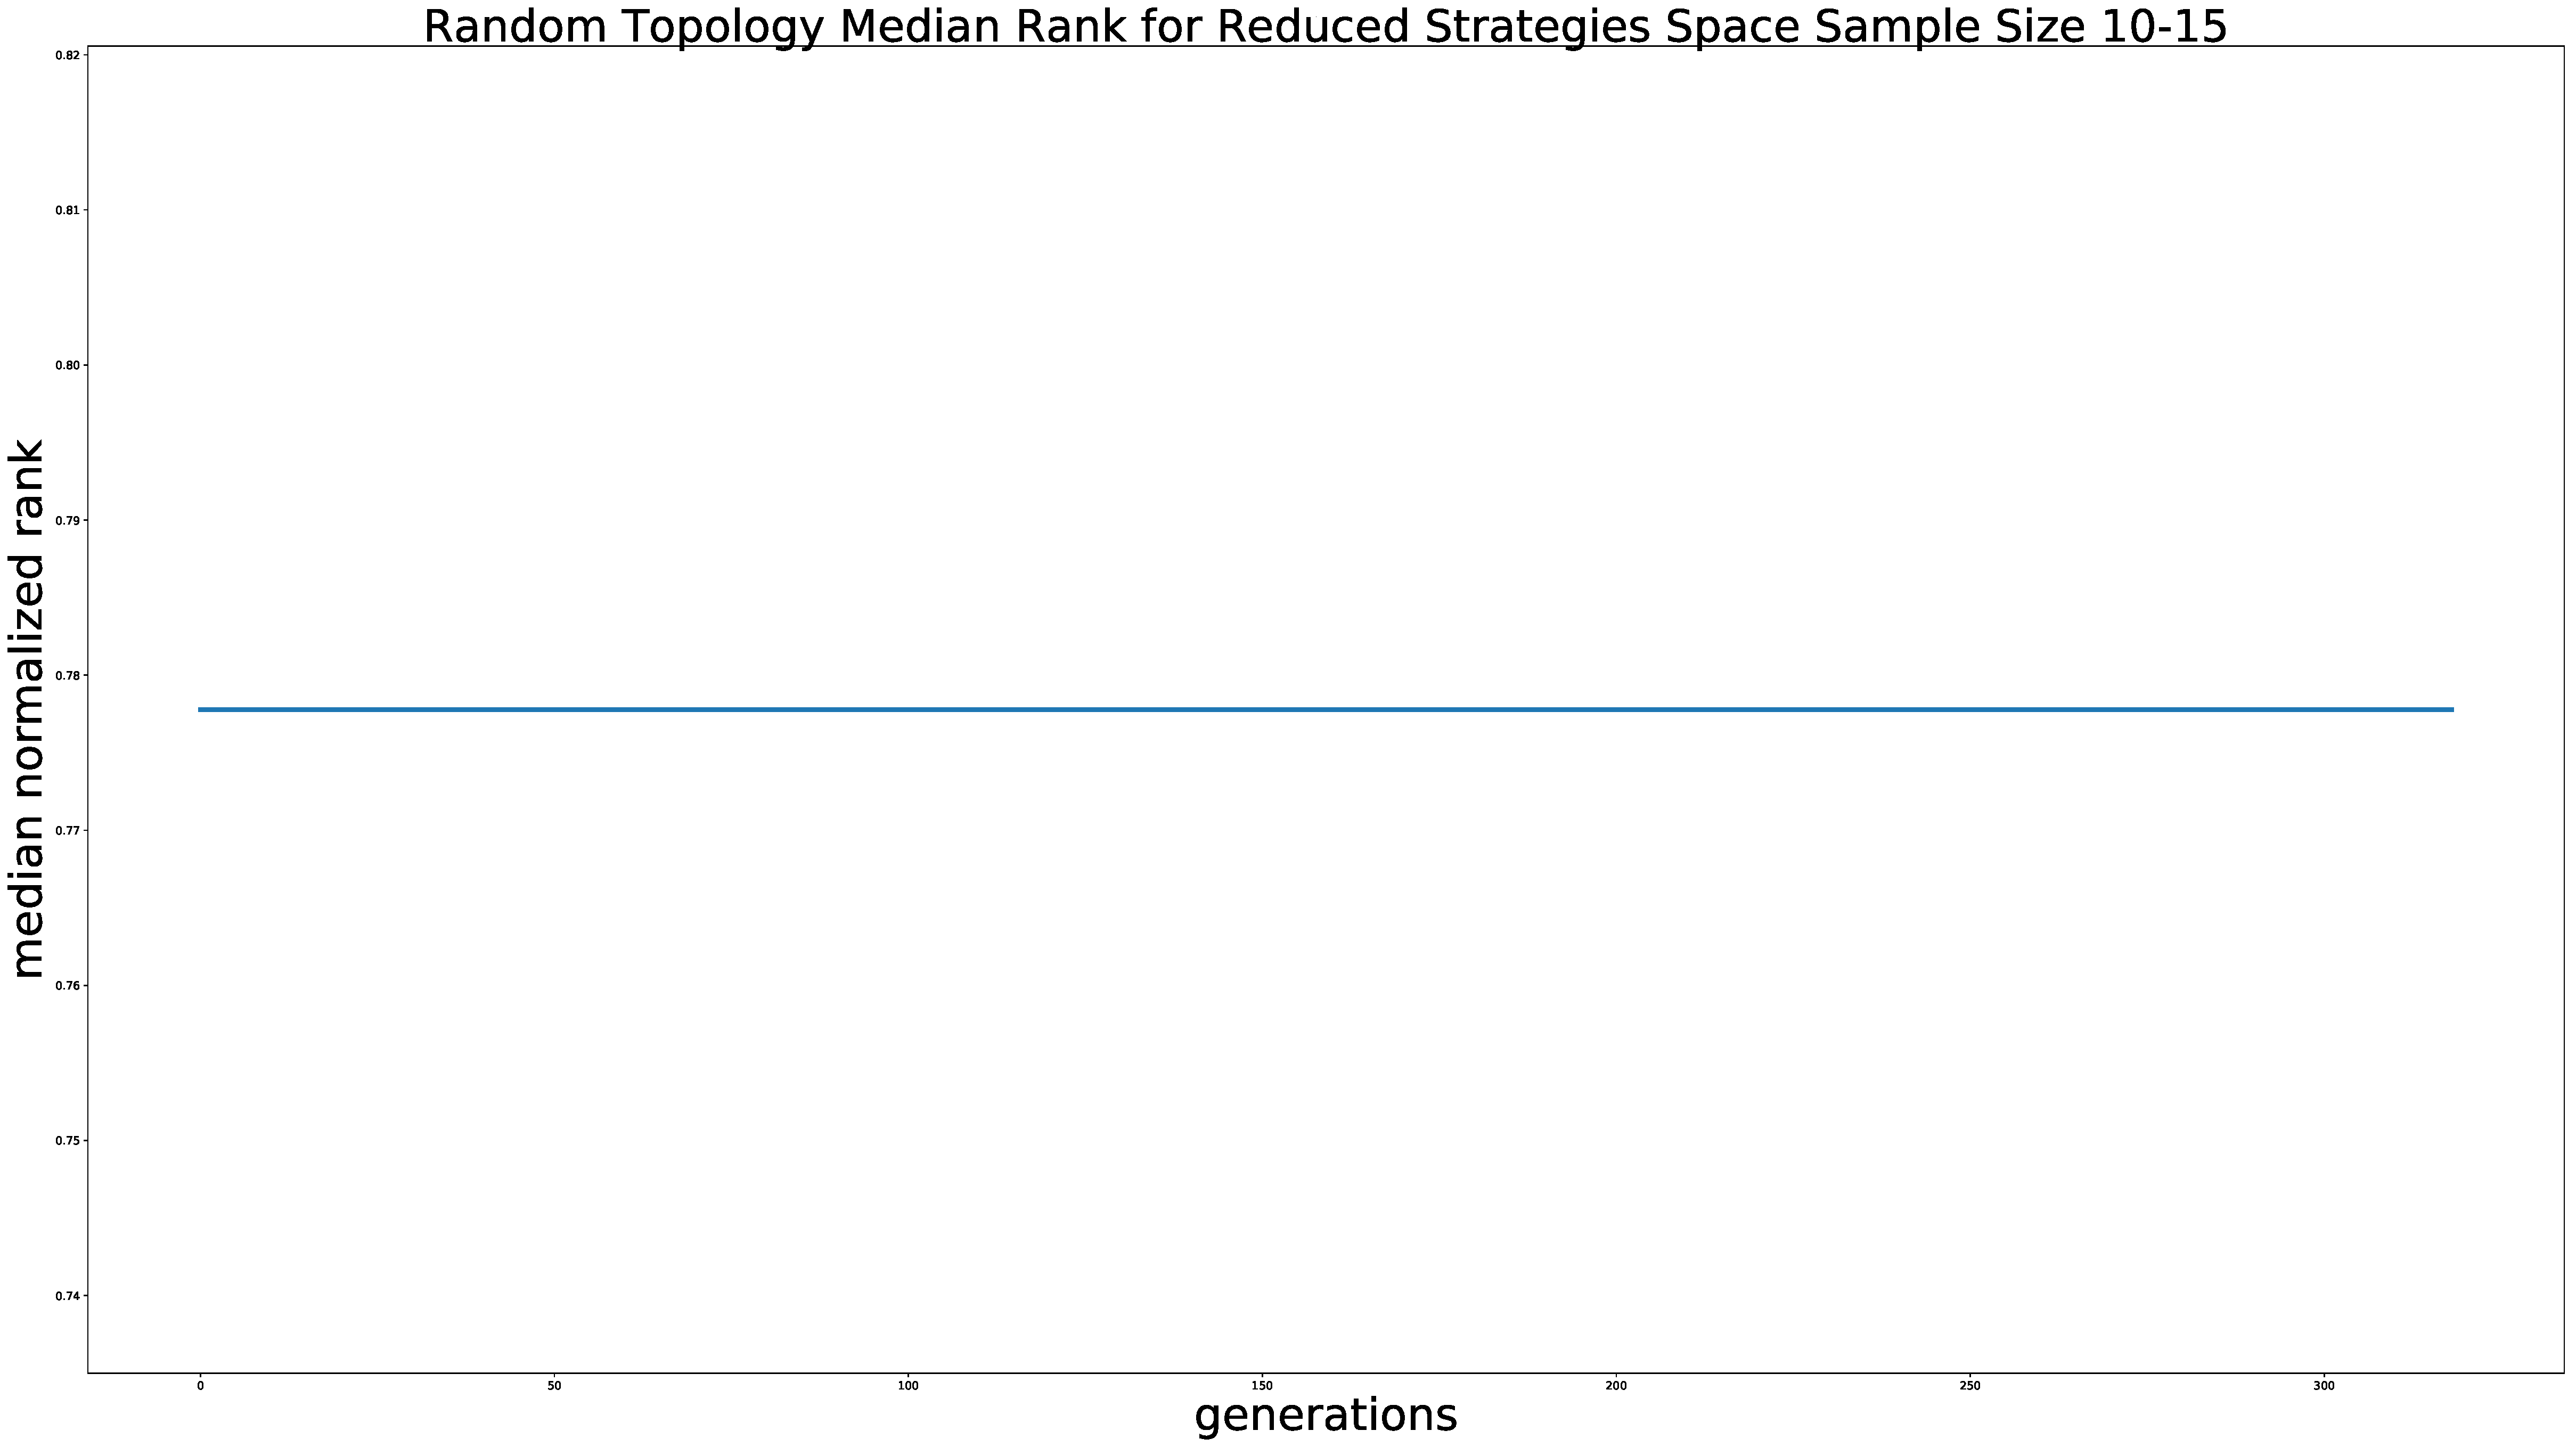
\includegraphics[width=\linewidth]{chapter-five/random-men-der.pdf}
		\caption{Only basic strategies}
	\end{subfigure}
	\hfill
	\begin{subfigure}[H]{0.45\textwidth}
		\centering
		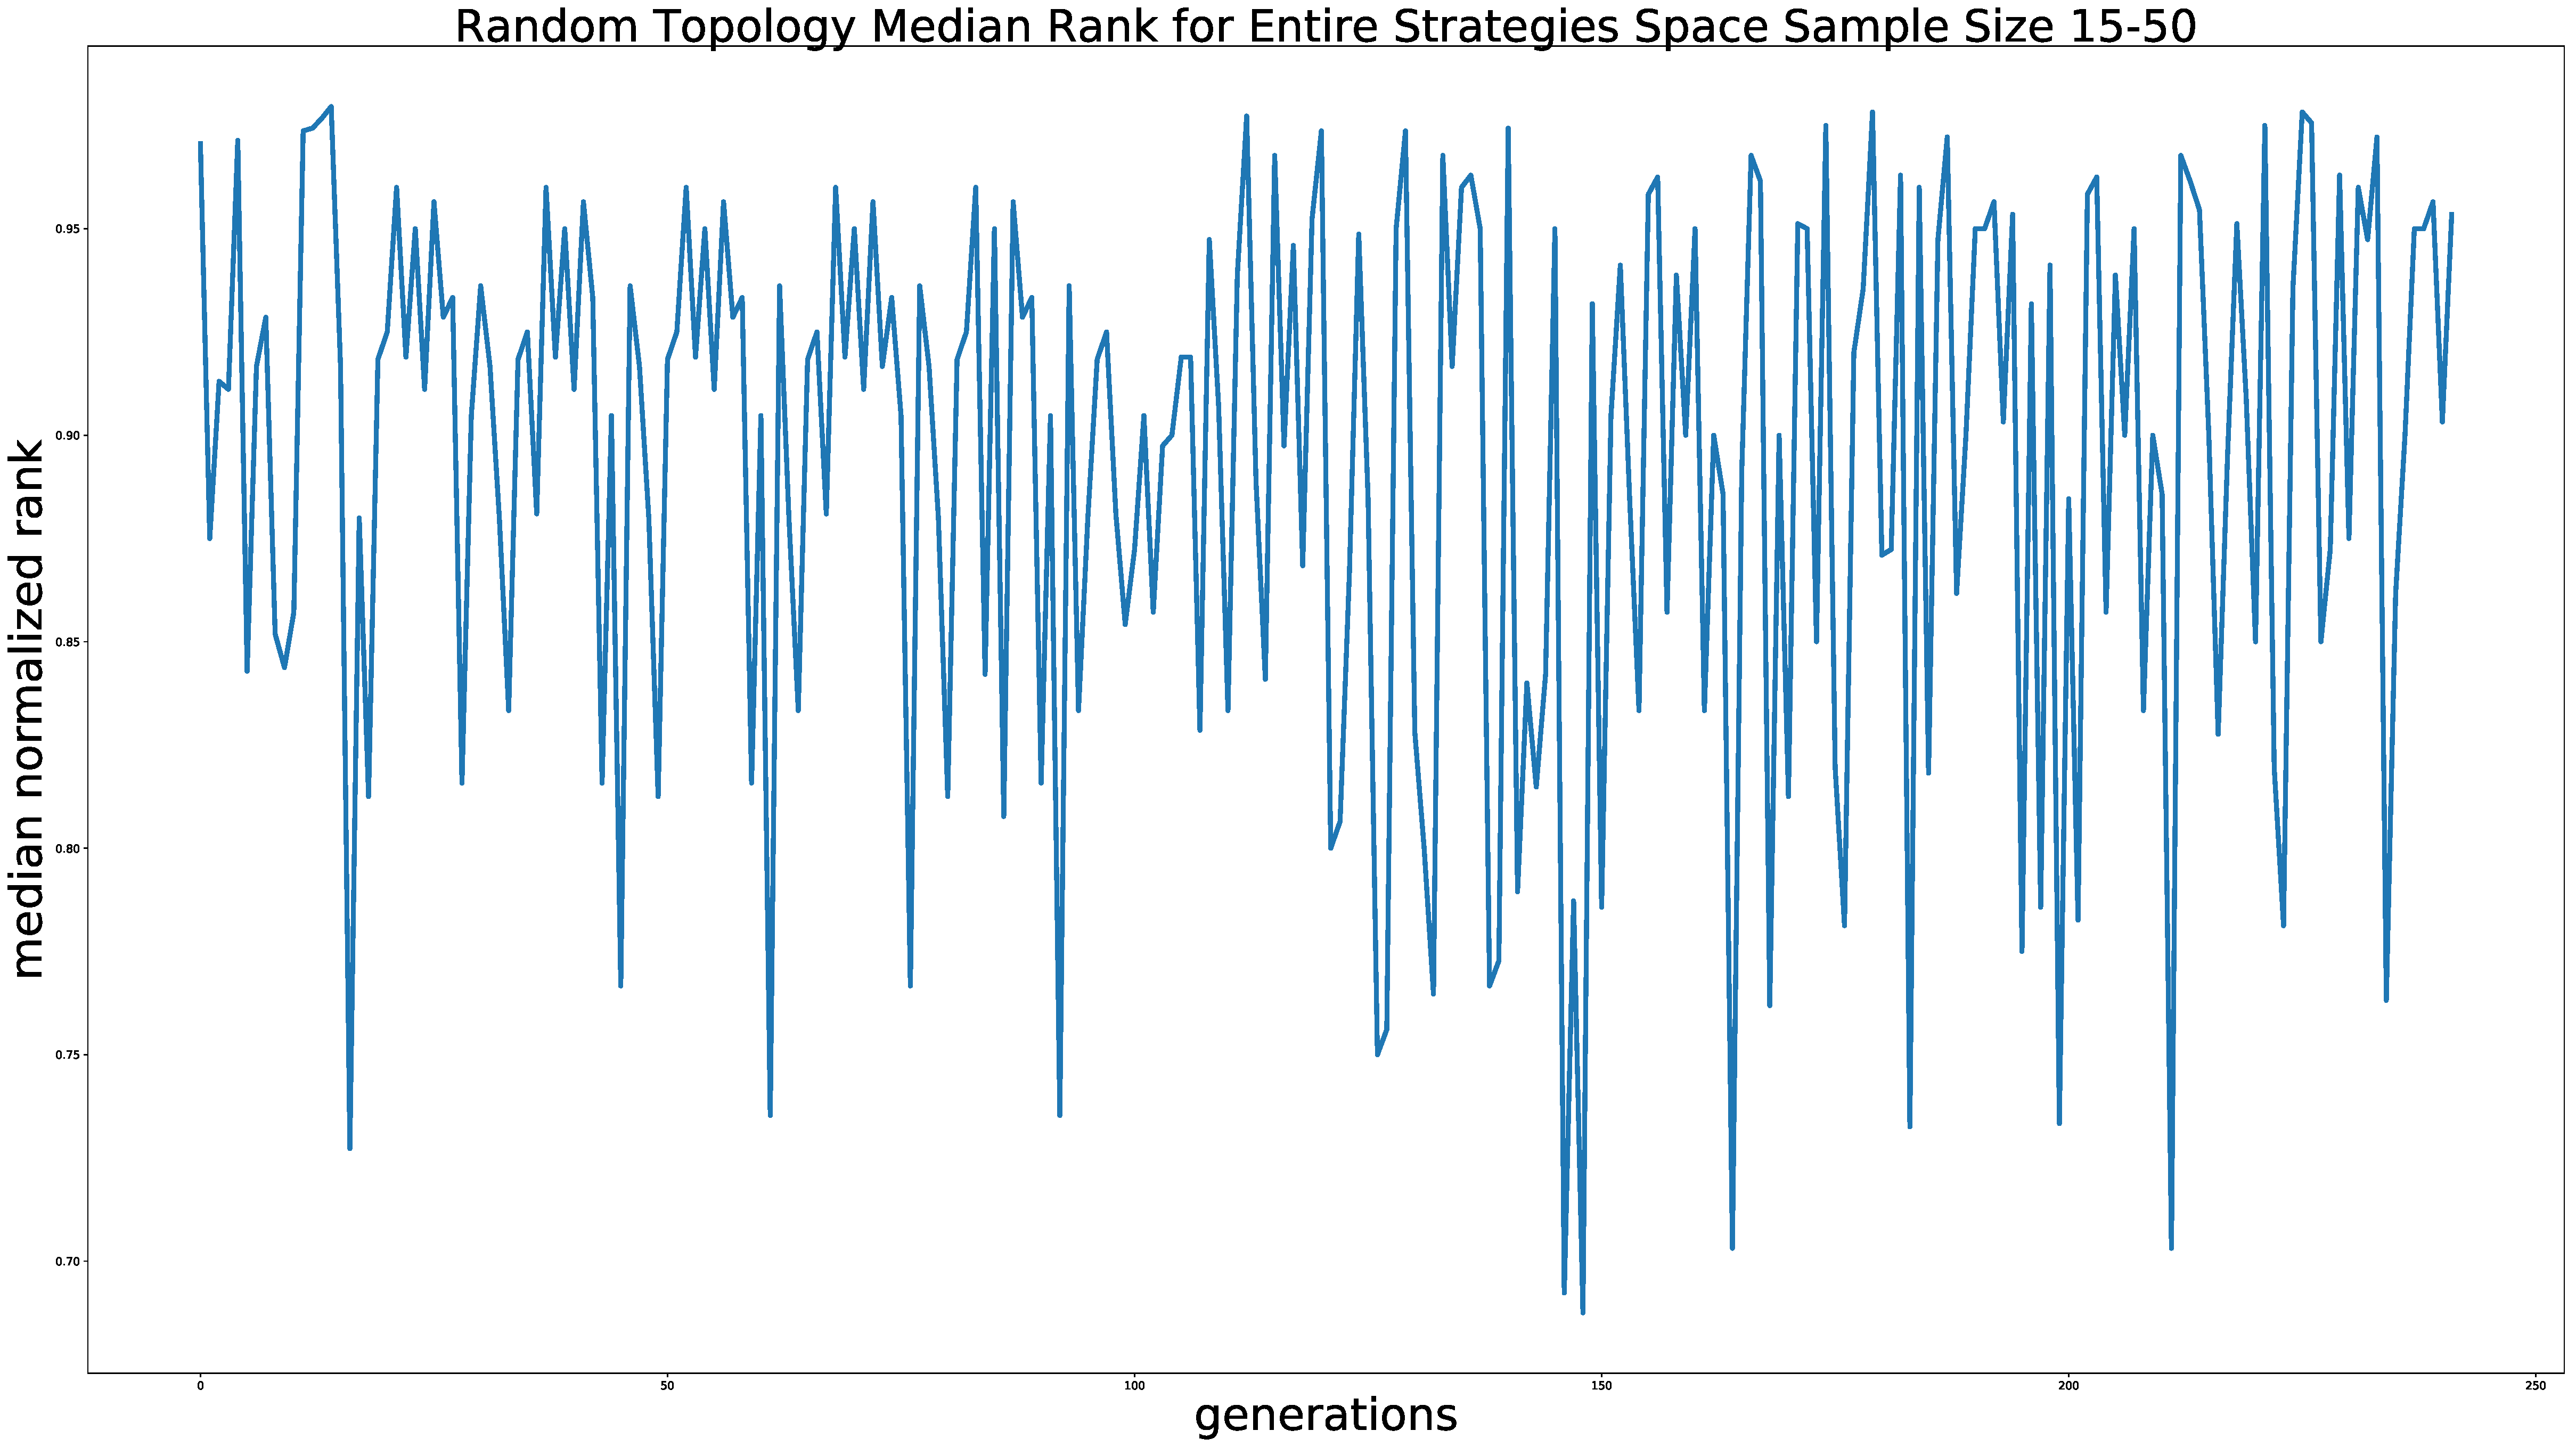
\includegraphics[width=\linewidth]{chapter-five/random-men-long.pdf}
		\caption{All strategies, sample size 10-15}
	\end{subfigure}
  \hfill
  \begin{subfigure}[H]{0.45\textwidth}
    \centering
    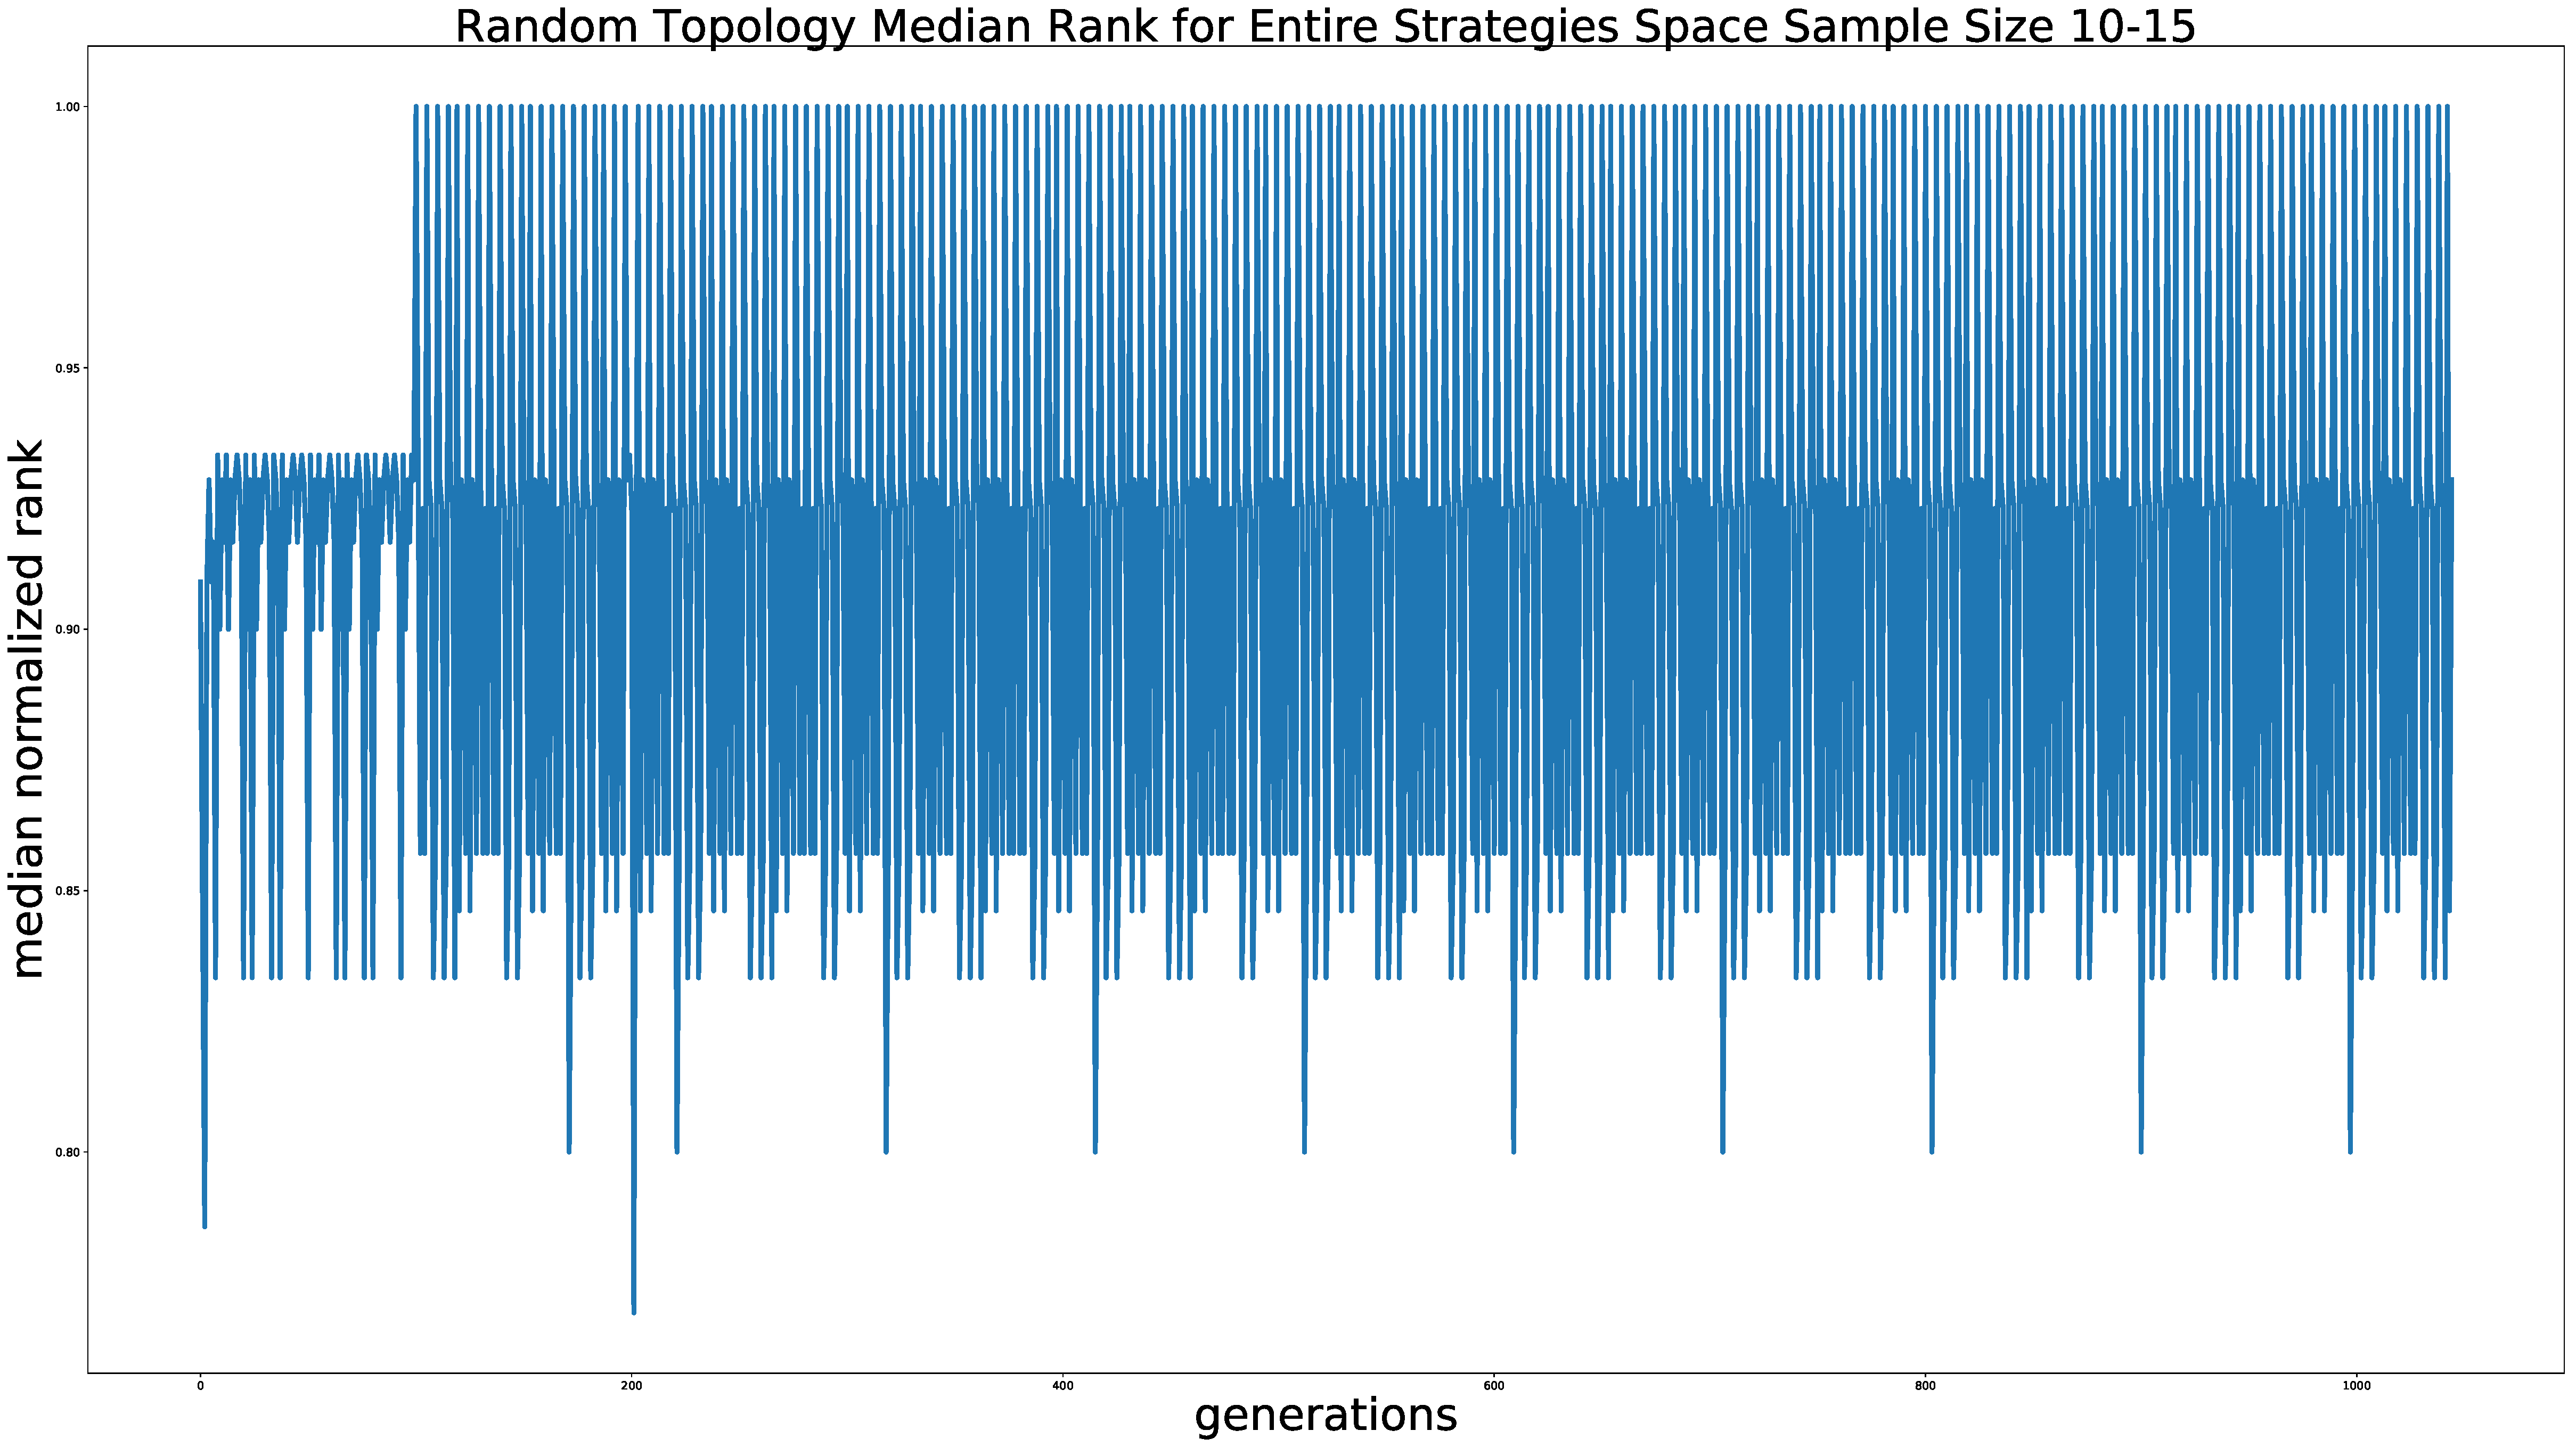
\includegraphics[width=\linewidth]{chapter-five/random-men-short.pdf}
    \caption{All strategies, sample size 15-50}
  \end{subfigure}
	\caption{Lines plot for the median normalized rank variation during the
          evolutionary algorithm}
	\label{fig:line-plots-median}
\end{figure}

For further research an extra algorithm has been performed. This time the
objective function has been measured as the minimum normalized score and was carried
out for only the entire strategy space. The results
that were generated from this run are given by the Table~\ref{results-min-geten}.
The overall results have been lower than before. The best score has been achieved for
a sample size of 15 to 50 and returned an minimum normalized score of 0.478.

\begin{table}[H]
\centering
\begin{adjustbox}{width=0.8\textwidth}
\small
\begin{tabular}{cccccccccc}
    \toprule
\multicolumn{4}{|c|}{\textbf{Results}}                                                                                                                                                                                             \\ \hline
                                     & lookup values  & generation   & score                                                                                                                                              \\ \hline
\begin{tabular}[c]{@{}l@{}}entire strategy space\\ sample size(5-15)\end{tabular}   & \begin{tabular}[c]{@{}l@{}}DDDDDCCDCDCDDCCDCCDDCCCDDCDCDCDC\\ CCCCCCDCDCDDDDCCDCDCDDDDDCDDDDCD\end{tabular} & 47 & 0.692308                  \\ \hline
                                     & \begin{tabular}[c]{@{}l@{}}CCDCDCDDDCCDDCDCDCDDCCDCDDCDDDCD\\ CDCCDCCDDDDDCCCDCCDDDCDCDDDCCCDD\end{tabular}  & 13 & 0.692308                                                             \\ \hline
                                     & \begin{tabular}[c]{@{}l@{}}DCCCDDCCCDDCDDDDDDCDDCCDCCDDCDDD\\ DDDDCDDDDCCDDDDCCDCCCDDDCCCCCCCC\end{tabular}  & 8 & 0.692308                                                             \\ \hline
\begin{tabular}[c]{@{}l@{}}entire strategy space\\ sample size(15-50)\end{tabular}& \begin{tabular}[c]{@{}l@{}}CDCCDDCDDDCCCDDDDCDCDCCDDCDCCDDD\\ DCDCCDCCCDDDCDDCDCDCDDCCCCCCDDDC\end{tabular} & 49 & 0.478261                     \\ \bottomrule
\end{tabular}
\end{adjustbox}
\caption{Results for spatial lookup evolve algorithm for minimum normalized rank}
\label{results-min-geten}
\end{table}

In Figure~\ref{fig:line-plot-min}, the course of the minimum normalized rank
for the entire strategy space cases is shown. For the run with a sample size of 10 to 15, there was
high variation of the minimum normalized score throughout. On the other hand, for a sample
size of 15 to 50, the minimum normalized score falls to a stable state approximately
after the 200\nth generation.

\begin{figure}[H]
	\centering
	\begin{subfigure}[H]{0.45\textwidth}
		\centering
		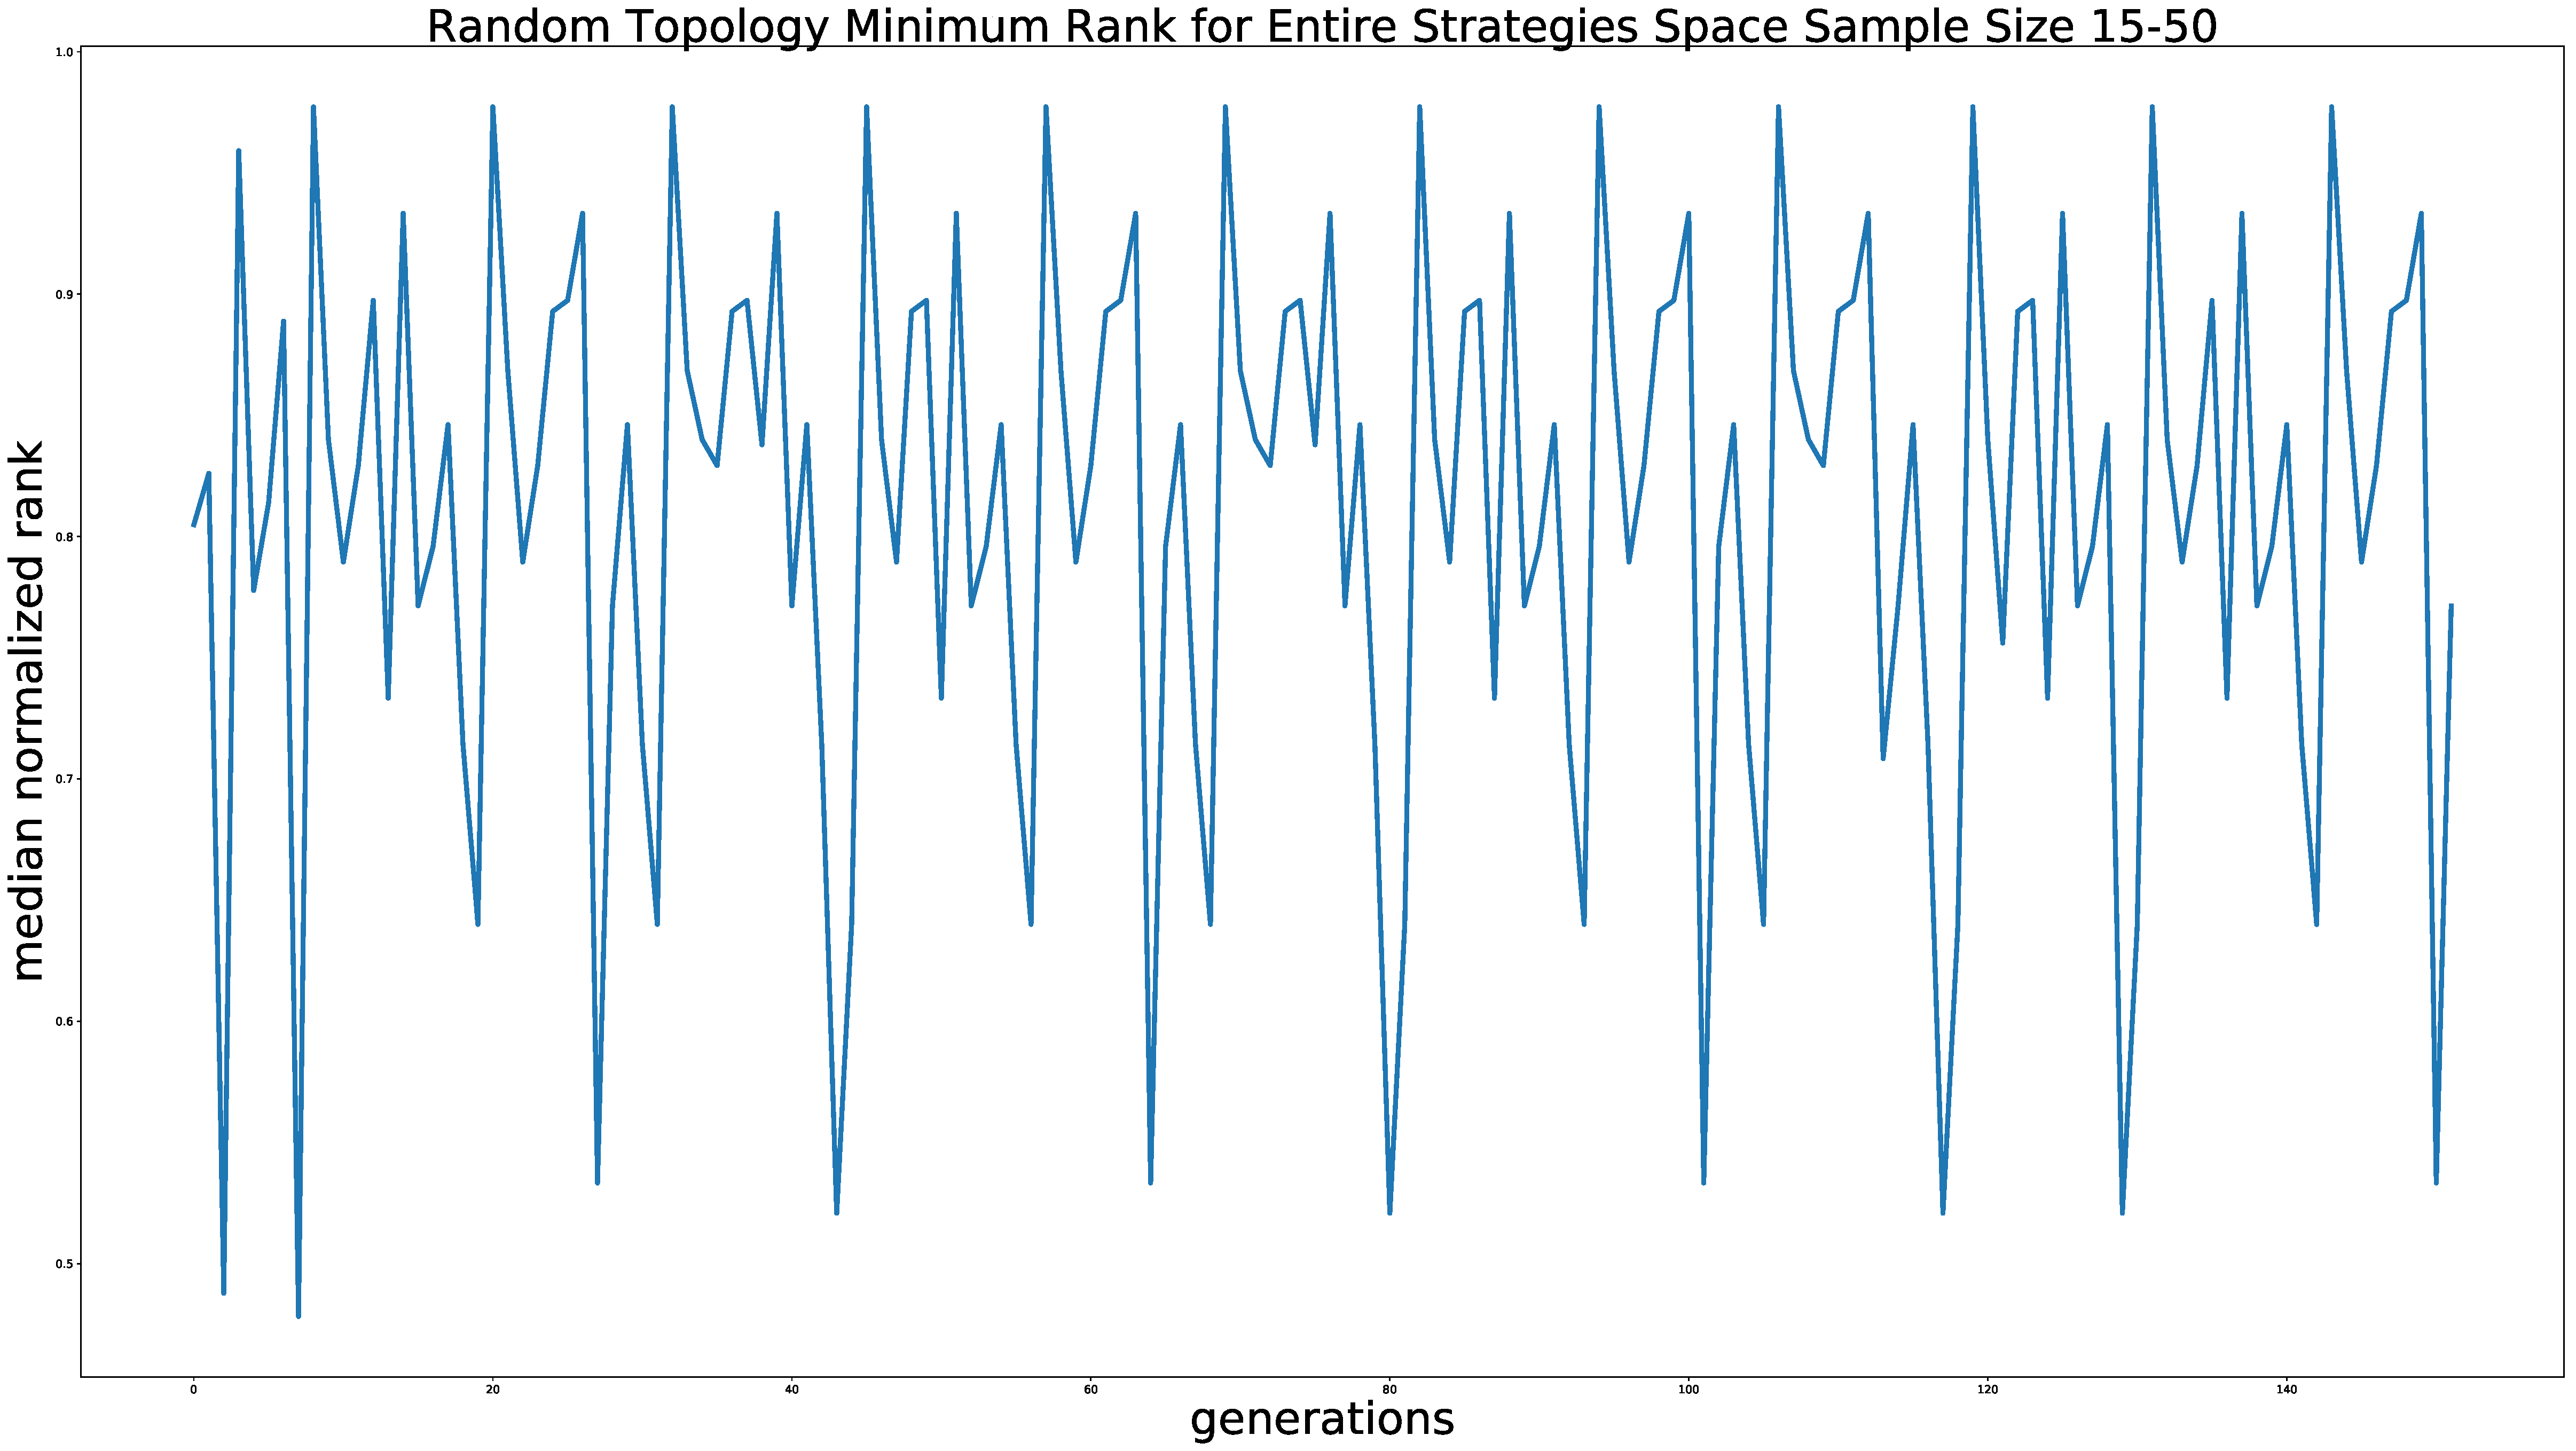
\includegraphics[width=\linewidth]{chapter-five/random-min-long.pdf}
		\caption{All strategies, sample size 10 to 15}
	\end{subfigure}
  \hfill
  \begin{subfigure}[H]{0.45\textwidth}
    \centering
    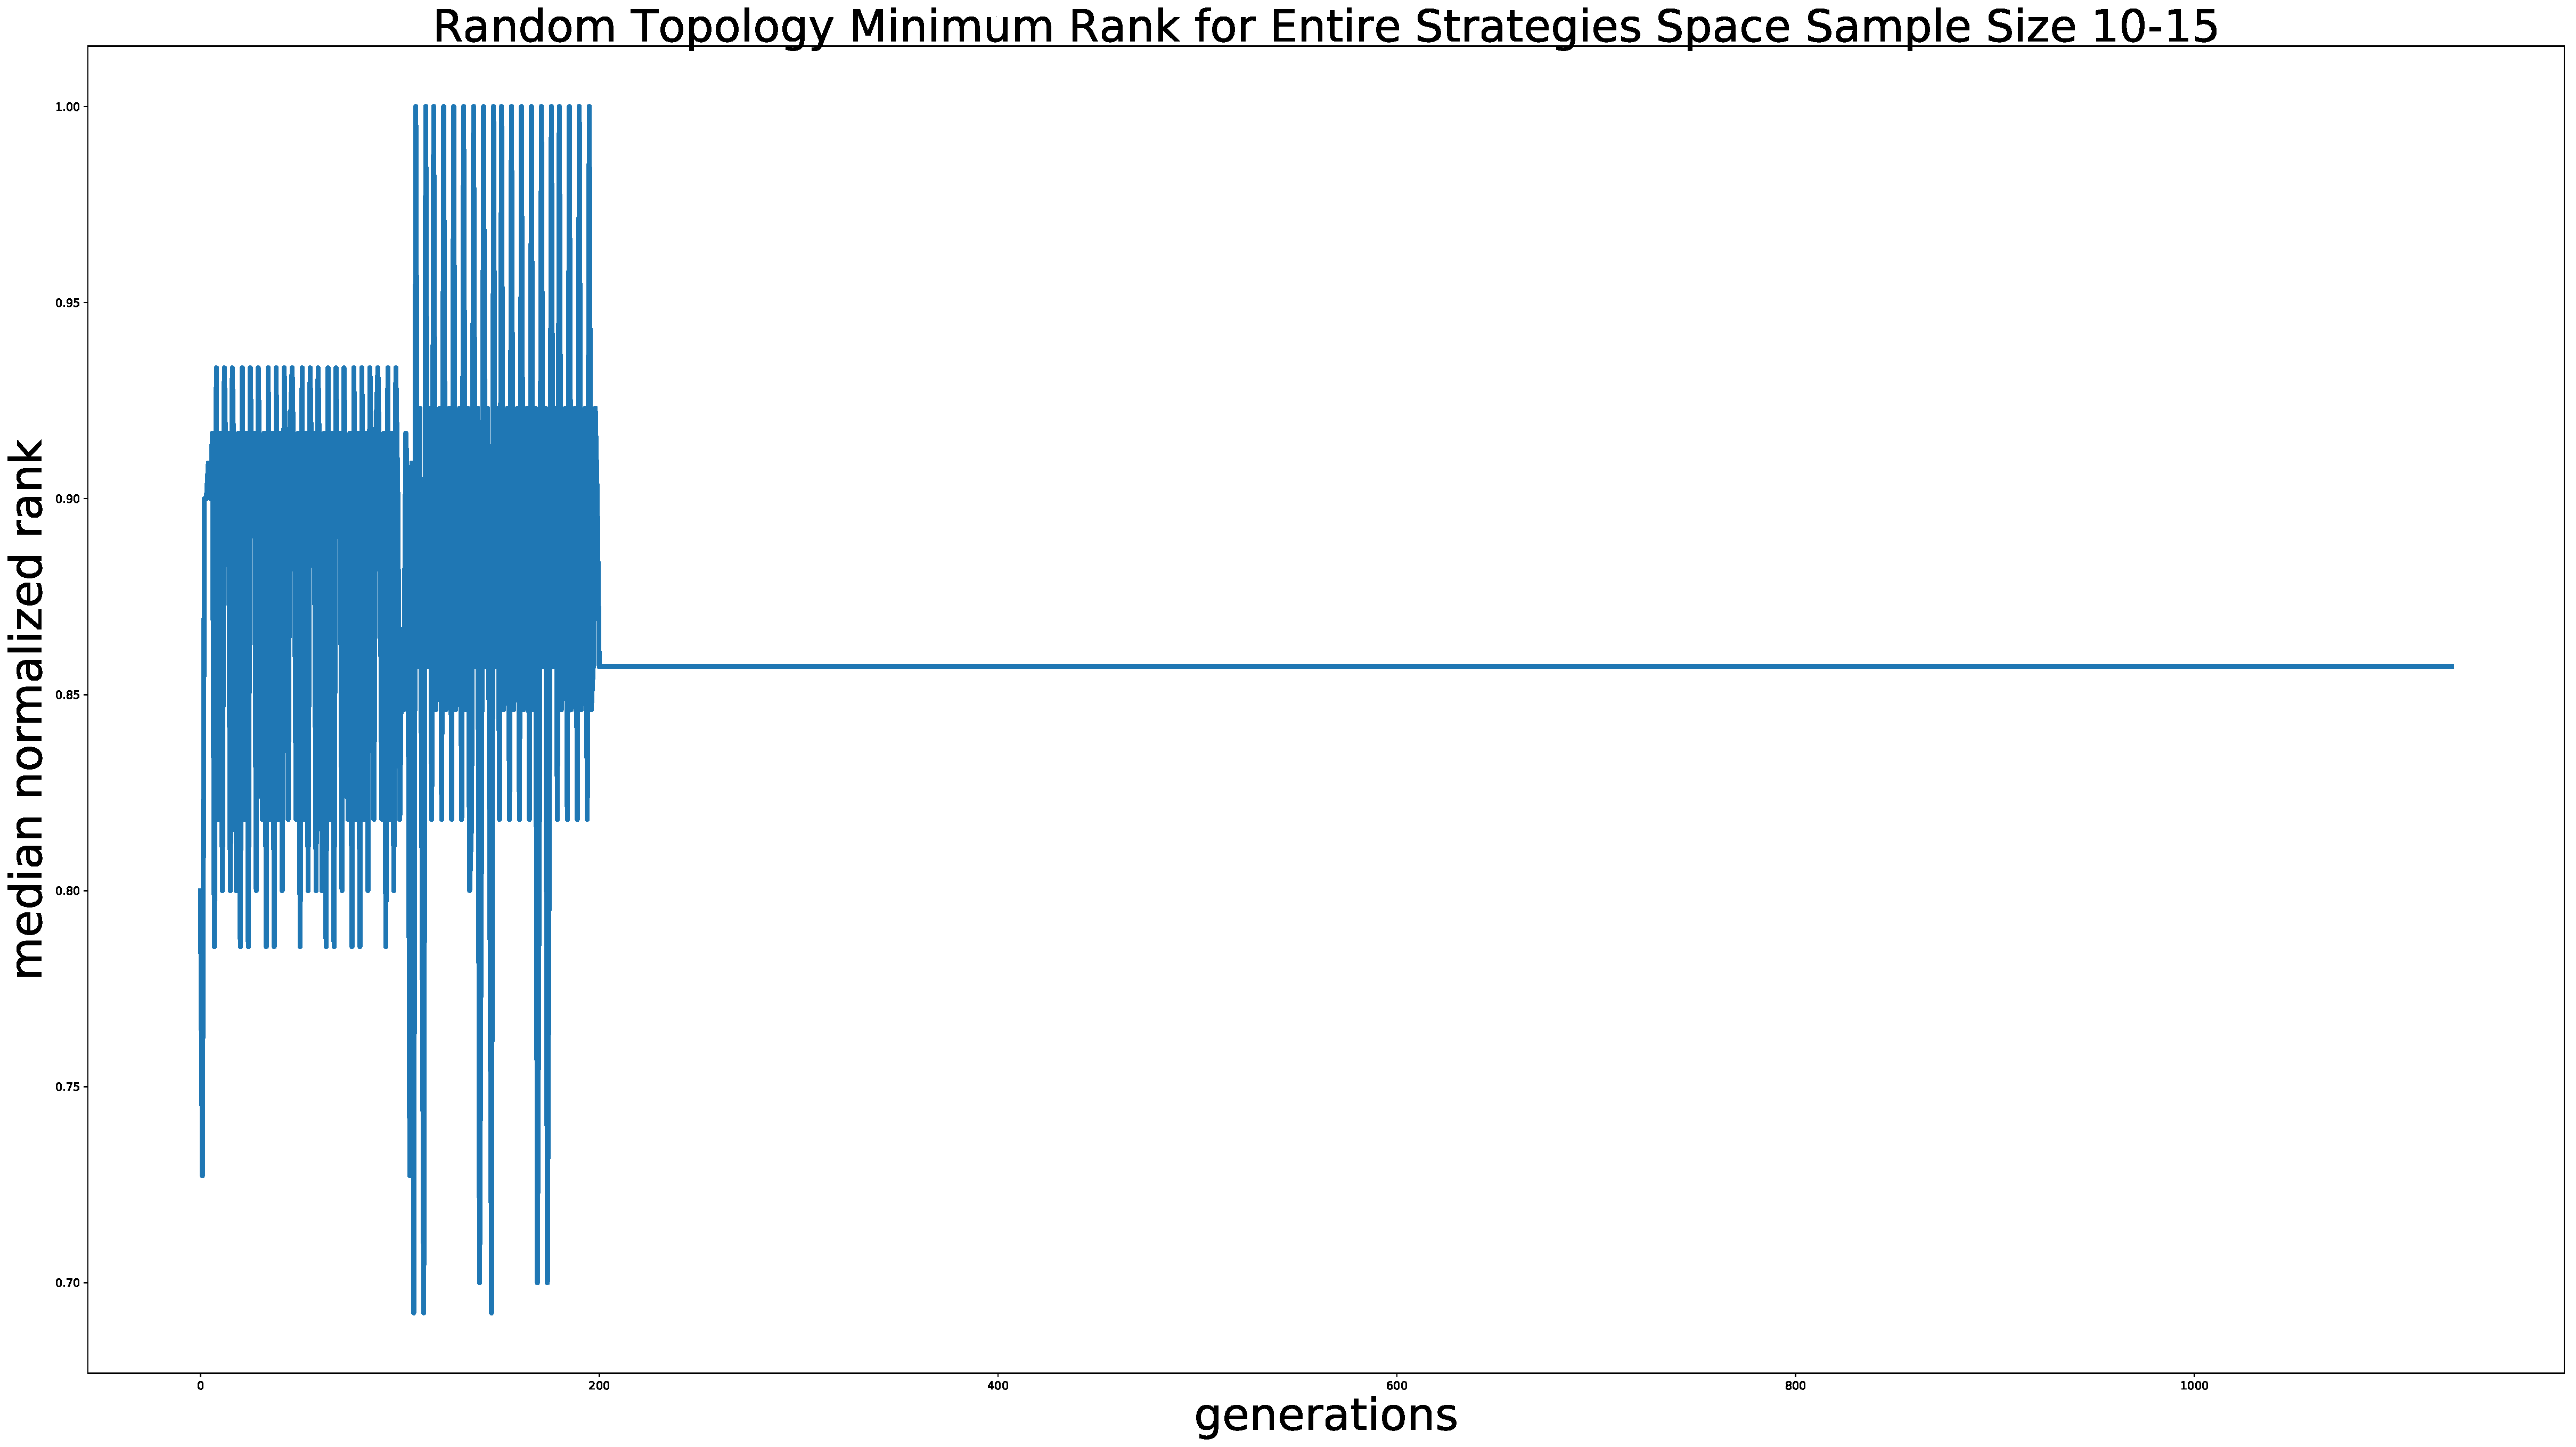
\includegraphics[width=\linewidth]{chapter-five/random-min-short.pdf}
    \caption{All strategies, sample size 15 to 50}
  \end{subfigure}
	\caption{Lines plot for the minimum normalized rank variation during the
          evolutionary algorithm}
	\label{fig:line-plot-min}
\end{figure}

In this section the lookup tables that have been produced by the spatial lookup
evolve algorithm from each case that has been implemented were presented and discussed.
The best lookup table for measuring the median normalized rank has been estimated
at 0.68 and for the second trial, where the minimum normalized rank was taken into
account, the algorithm returned a score of 0.478.

In the experiment performed and analyzed in \autoref{chap:Four}, Gradual has been
the best performed strategy based on the median normalized rank. The strategy in
particularly achieved a median normalized rank of 0.23. In both trials of the
spatial evolve algorithm it can been seen that the LookerUp strategy did not
manage to score less than that. Even so, the algorithm was performed for a small
number of generations. It would be valuable to perform all the experiments of
\autoref{chap:Four} with these newly trained strategies however time constraints have not
permitted this.

The following section, briefly summarizes the results returned by the algorithm
for some extra cases. This has been done mainly for comparison reasons
and in these cases each of the three complex networks are studied individually.

\section{Further Results}
\label{sub:futher-results}
In this section some additional results of the spatial lookup evolve algorithm
are discussed. In the previous section the networks used in the scoring process
have been randomly picked between small world, random and complete networks.
In this section the algorithm has been performed for each of networks individually
using the objective function of the median normalized rank.

This was implemented mainly to identify whether a well performed strategy
exists for a specific spatial tournament. Table~\ref{deter-indiv} and Table~\ref{non-deter-indiv} summarize the results.

For the reduced strategy space case where the topology of the spatial tournaments has been
a Watts Strogatz network, the first rate lookup table achieved a median normalized
score of 0, in the 635\nth generation. Moreover, for the Erd\"{o}s R\'{e}nyi
topology the best lookup table has a score of 0.5 in the 1399\nth generation, similarly
to the complete network where the lowest rank achieved was 0.556.

\begin{table}[H]
\centering
\begin{adjustbox}{width=0.8\textwidth}
\small
\begin{tabular}{cccccccccc}
    \toprule
\multicolumn{4}{|c|}{\textbf{Reduced strategy space}}                                                                                                         \\ \hline
                       & lookup                                                                                                      & generation & score    \\ \hline
Watts Strogatz         & \begin{tabular}[c]{@{}l@{}}CDCCCDDDCCCDCCCDDDCDCDCCDCCCDCDCC\\ DCCDDDDCCCDDCDDCDDDDDDCCDDDDCDC\end{tabular} & 635        & 0.00     \\ \hline
Erd\"{o}s R\'{e}nyi    & \begin{tabular}[c]{@{}l@{}}CCCDDCCCDCDCCCCDDCCCCDDDDCCDCDCDD\\ DDCCCCCDDCCCDDCDCCDCDCDDDCDCDCC\end{tabular} & 1399       & 0.5      \\ \hline
Complete               & \begin{tabular}[c]{@{}l@{}}DDCCCCDDDDDDCCDCCDDDCDDDCCDDDDCC\\ DCCDDCDCCCCDCCDDDCCDCCDCDCCCCCCC\end{tabular} & 1299       & 0.555556 \\ \hline
\end{tabular}
\end{adjustbox}
\caption{Results using only the basic strategies for Watts Strogatz, Erd\"{o}s R\'{e}nyi and complete networks}
\label{deter-indiv}
\end{table}

Furthermore, the results for the entire strategy space population are
shown in Table~\ref{non-deter-indiv}. For a sample size between 10 to 15 the
best scores are 0.818 for the Watts Strogatz network, 0.714 for the Erd\"{o}s R\'{e}nyi
network and 0.769 for the complete. Similarly, for a sample size of 15 to 50.
For the Watts Strogatz network the lowest median rank has been 0.810, for the Erd\"{o}s R\'{e}nyi
network 0.656 and finally 0.739 for the complete. Significant higher, now that the
all strategies have been added to the tournaments.

\begin{table}[H]
  \centering
  \begin{adjustbox}{width=0.8\textwidth}
  \small
  \begin{tabular}{cccccccccc}
      \toprule
\multicolumn{5}{|c|}{\textbf{Entire strategy space}}                                                                                                                                       \\ \hline
                        & sample size & lookup                                                                                                      & generation & score                     \\ \hline
Watts Strogatz          & 10- 15       & \begin{tabular}[c]{@{}l@{}}DDDDCCCCDCDDCDCDCCDCCDCDCCDCCCCC\\ DCCDCDCCCCDCDCCDDDCCCCCCDDCDCCDD\end{tabular} & 199        & 0.818                     \\ \hline
                        & 15 - 50     & \begin{tabular}[c]{@{}l@{}}DDCCCDDCDCDDCDCCDCCDDCCDCCDDCDCD\\ CDDCCDDDCCCDCDCDCDDDDCDDDDDCCDDC\end{tabular} & 59         & 0.810                     \\ \hline
Erd\"{o}s R\'{e}nyi     & 10 - 15      & \begin{tabular}[c]{@{}l@{}}DCCDDCDDDCDDCDDCCDDDDDDCDDDCCCDC\\ CCCDCDCDDDDCCDCDCCDDCCCDDDCCDDCC\end{tabular} & 302        & 0.714                     \\ \hline
                        & 15 - 50     & \begin{tabular}[c]{@{}l@{}}DCCDDDDCCCCDDDCCDDCDCCDCCDCCCCCC\\ CDCDDDDCDDDDDCDDCCCCCDCCCCCDCDDC\end{tabular} & 11         & 0.656                     \\ \hline
Complete                & 10 - 15      & \begin{tabular}[c]{@{}l@{}}CCDCCDDDDCCCCCDDDDDCCDCCDCCCCCDD\\ DCCDCCCDCCDDDCDDDDDDCDDDCDDCDDCD\end{tabular} & 202        & \multicolumn{1}{r}{0.769} \\ \hline
                        & 15 - 50     & \begin{tabular}[c]{@{}l@{}}CCCDDCDCCDCDCDDCDCDDCCCDCDCDDCCC\\ DDDDDDCCCDCCDDDDCDCDDDCCCDDDCDCC\end{tabular} & 13         & 0.736                     \\ \bottomrule
\end{tabular}
\end{adjustbox}
\caption{Results using all 132 strategies for Watts Strogatz, Erd\"{o}s R\'{e}nyi and complete networks}
\label{non-deter-indiv}
\end{table}

In the Appendix~\ref{append:genetic-variation} the line plots of the score variation
for the further results are illustrated. Figure~\ref{fig:line-plots-individuals-all-short}
shows that even for the for the reduced strategy space case variation exists but
significantly less than those of the entire strategy space.
Figure~\ref{fig:line-plots-individuals-all-short} and Figure~\ref{fig:line-plots-individuals-all-long}
illustrate the plots for the entire strategy space, where similarly to \autoref{sub:results}
have a high variation.

In conclusion, the average scores did not differ much for the results returned
in ~\autoref{sub:results} and most of the LookerUp strategies did not manage to
beat the median rank of Gradual. This holds for all but one. The achievement
of this section has been that for a spatial tournament of a small world topology,
where only the basic strategies participated a winning strategy has managed to be trained.
The lookup table returned a median normalized score of 0, thus the strategy has been winning the spatial tournaments.
These results are a proof of concept that winning strategies for spatial tournaments
do exist. To further research this the spatial algorithm would have to be re performed
for a larger number of generations.
